\subsection{Causal models}\label{sec:causal}

This sequence of models of joint independence has another
interpretation when the ordering of the variables is based on a set
of ordered hypotheses involving causal relationships among
variables 
(\citet{Goodman:73}, \citet[\S 7.2]{Fienberg:80}).  Suppose, for example,
that the causal ordering of four variables is \(A \rightarrow B
\rightarrow C \rightarrow D\), where the arrow means ``is antecedent
to.''  Goodman suggests that the conditional joint probabilities of
$B$, $C$, and $D$ given $A$ can be characterized by a set of
recursive logit models which treat
\begin{seriate}
\item $B$ as a response to $A$,
\item $C$
as a response to $A$ and $B$ jointly,
\item and $D$ as a response to $A$,
$B$ and $C$.
\end{seriate}
These are equivalent to the log-linear models which
we fit as the sequential baseline models of joint independence,
namely \LLM{A,B}, \LLM{AB,C}, and \LLM{ABC,D}.  The combination of these
models with the marginal probabilities of A gives a characterization
of the joint probabilities of all four variables.

\begin{Example}[marital1]{Marital status and pre- and extramarital sex}

A study of divorce patterns  by \citet{ThornesCollard:79} reported
the \(2^4\) table shown in  
\tabref{tab:maridat} (see \datref{dat:marital} for the SAS \Dset).
These data were analysed by \citet[\S 7.2.4]{Agresti:90}
and by \citet{Friendly:94a}, from which this account draws.
A sample of
about 500 people who had petitioned for divorce, and a similar number
of married people were asked two questions regarding their pre- and
extramarital sexual experience:  (1) ``Before you married your
(former) husband/wife, had you ever made love with anyone else?,''
(2) ``During your (former) marriage (did you) have you had any
affairs or brief sexual encounters with another man/woman?'' 
The
table variables are thus gender ($G$), reported premarital ($P$)
and extramarital ($E$) sex, and current marital status ($M$).


%%
%% Table marital written by md2tex 01MAY98 13:11
%%
\begin{table}[htb]
 \caption{Marital Status in Relation to Gender and Reported Premarital and Extramarital Sex}
 \label{tab:maridat}
 \begin{center}
  \begin{tabular}{|lll|rr|}
   \hline
{\bfseries\large Extramarital} & {\bfseries\large Premarital} &  & \multicolumn{2}{c|}{\bfseries\large Marital Status}\rule{0in}{2.5ex}\\
{\bfseries\large Sex} & {\bfseries\large Sex} & {\bfseries\large Gender} & Divorced  & Married   \\
   \hline
Yes            & Yes          & Women    &         17 &          4 \\
No             &              &          &         54 &         25 \\
[4pt]
Yes            & No           &          &         36 &          4 \\
No             &              &          &        214 &        322 \\
[4pt]
Yes            & Yes          & Men      &         28 &         11 \\
No             &              &          &         60 &         42 \\
[4pt]
Yes            & No           &          &         17 &          4 \\
No             &              &          &         68 &        130 \\
   \hline
\rule{0in}{2.5ex}{\bfseries\large Total} & & &       494 &        542 \\
   \hline
  \end{tabular}
 \end{center}
\end{table}


In this analysis we consider the variables in the order $G$, $P$,
$E$, and $M$.  That is, the first stage  treats $P$ as a
response to $G$ and examines the [Gender][Pre] mosaic to assess
whether gender has an effect on premarital sex.  The second stage
treats $E$ as a response to $G$ and $P$ jointly;  the
mosaic for [Gender, Pre] [Extra] shows whether extramarital sex
is related to either gender or premarital sex.  Finally, the mosaic
for [Gender, Pre, Extra] [Marital] is examined for evidence of the
dependence of marital status on the three previous variables jointly.
As noted above, these models are equivalent to the
recursive logit models whose path diagram is \(G \rightarrow P
\rightarrow E \rightarrow M\).%
\footnote{ \citet[\S 7.2.4]{Agresti:90} considers a slightly more complex,
but more realistic model in which premarital sex affects both the propensity
to have extramarital sex and subsequent marital status.}
The \(G^2\) values for these models
shown below provide a decomposition of the
\(G^2\) for the model of complete independence fit to the full table.

\begin{center}
 \begin{tabular}{rrr}
 \hline
  Model        & df & \(G^2\) \\ 
 \hline
  \llmtwo{G}{P}    & 1  & 75.259 \\ 
  \llmtwo{GP}{E}   & 3  & 48.929 \\ 
  \llmtwo{GPE}{M}  & 7  & 107.956 \\ 
 \hline
  \llmfour{G}{P}{E}{M} & 11 & 232.142 \\ 
 \hline
 \end{tabular}
\end{center}

The [Gender] [Pre] mosaic is shown in \figref{fig:mosaic51}.
The mosaic shows that men are much more likely to report
premarital sex than are women; the sample odds ratio is 3.7.  We
also see that women are about twice as prevalent as men in this
sample.

%% two figures side-by-side
\begin{figure}[htb]
 \begin{minipage}[b]{.49\linewidth}
  \centering
  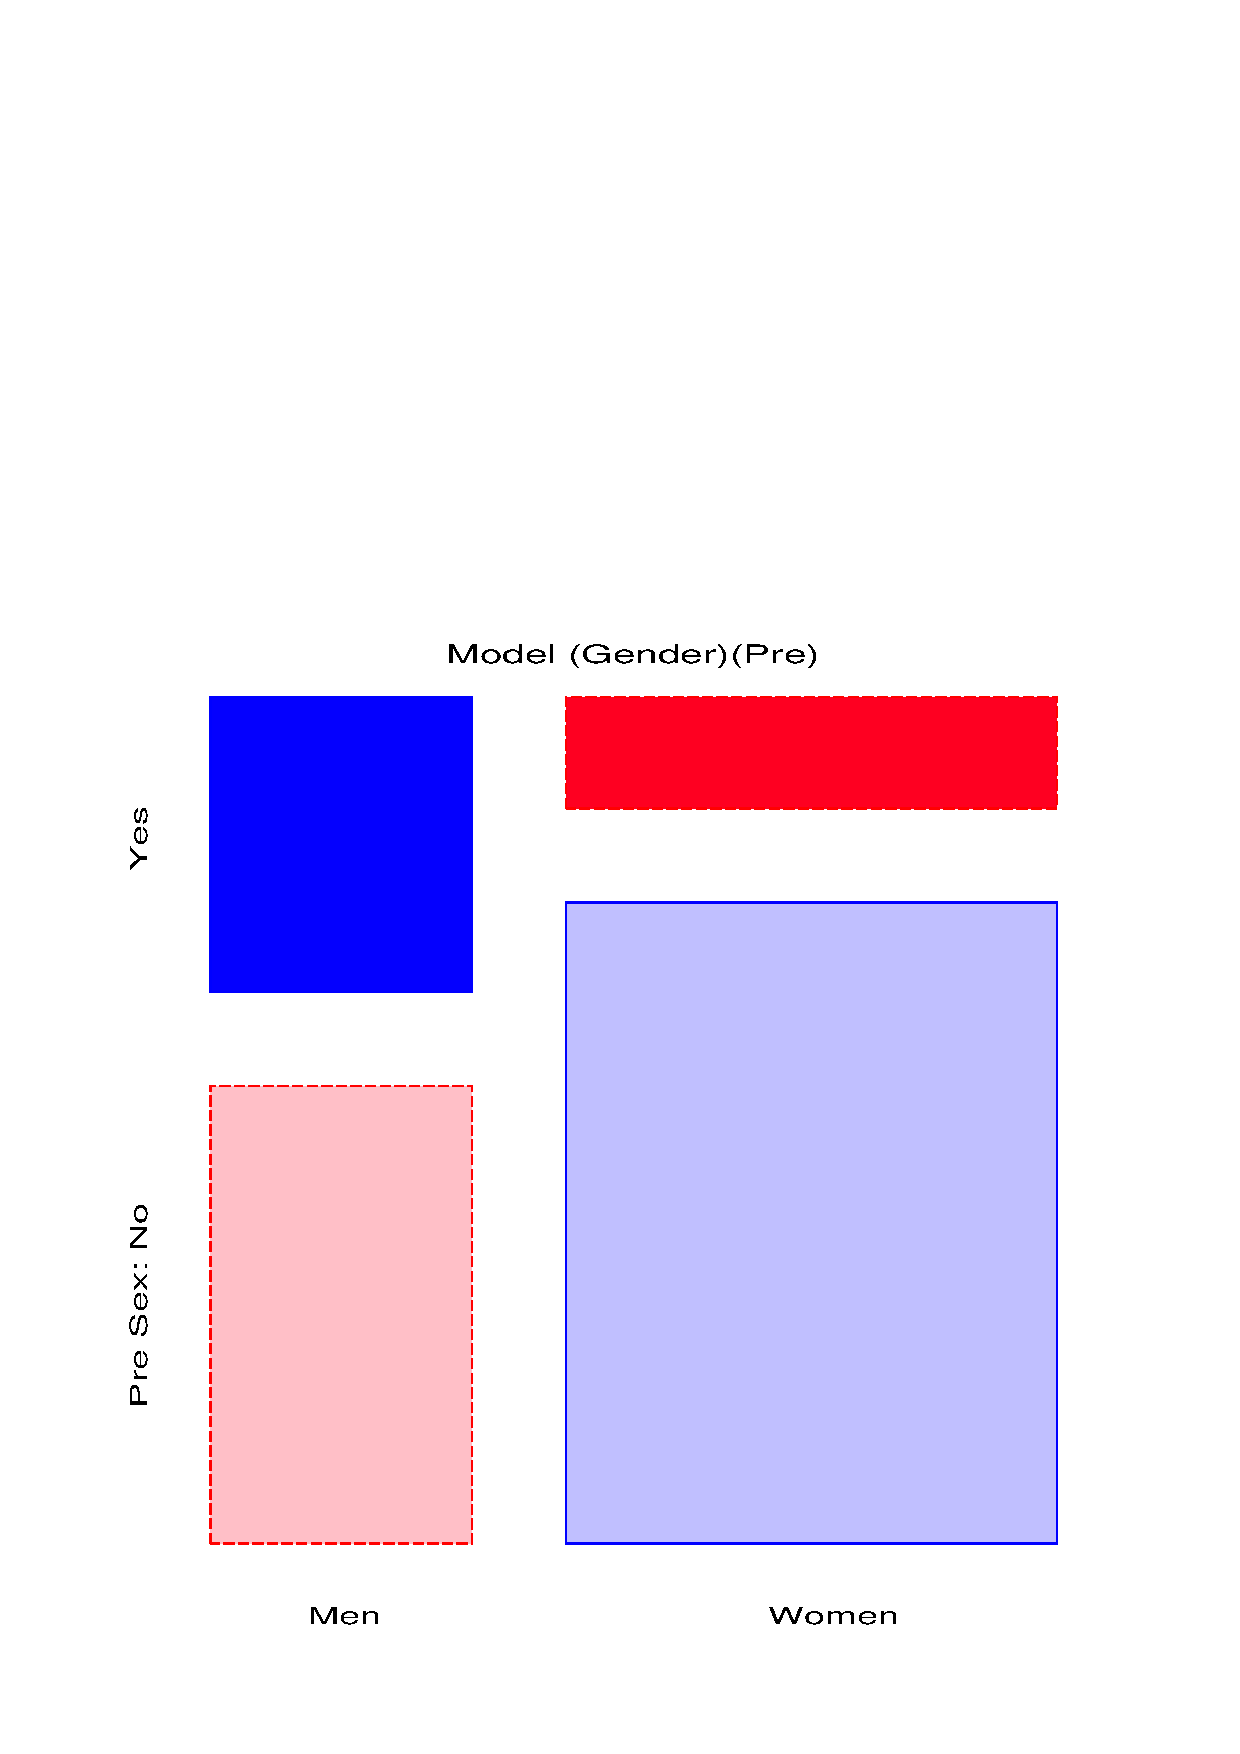
\includegraphics[width=1\linewidth]{ch4/fig/mosaic51}
  \caption[Mosaic display for gender and
pre-martial sexual experience]{Mosaic display for gender and
pre-martial sexual experience.}%
  \label{fig:mosaic51}
 \end{minipage}%
 \hfill
 \begin{minipage}[b]{.49\linewidth}
  \centering
  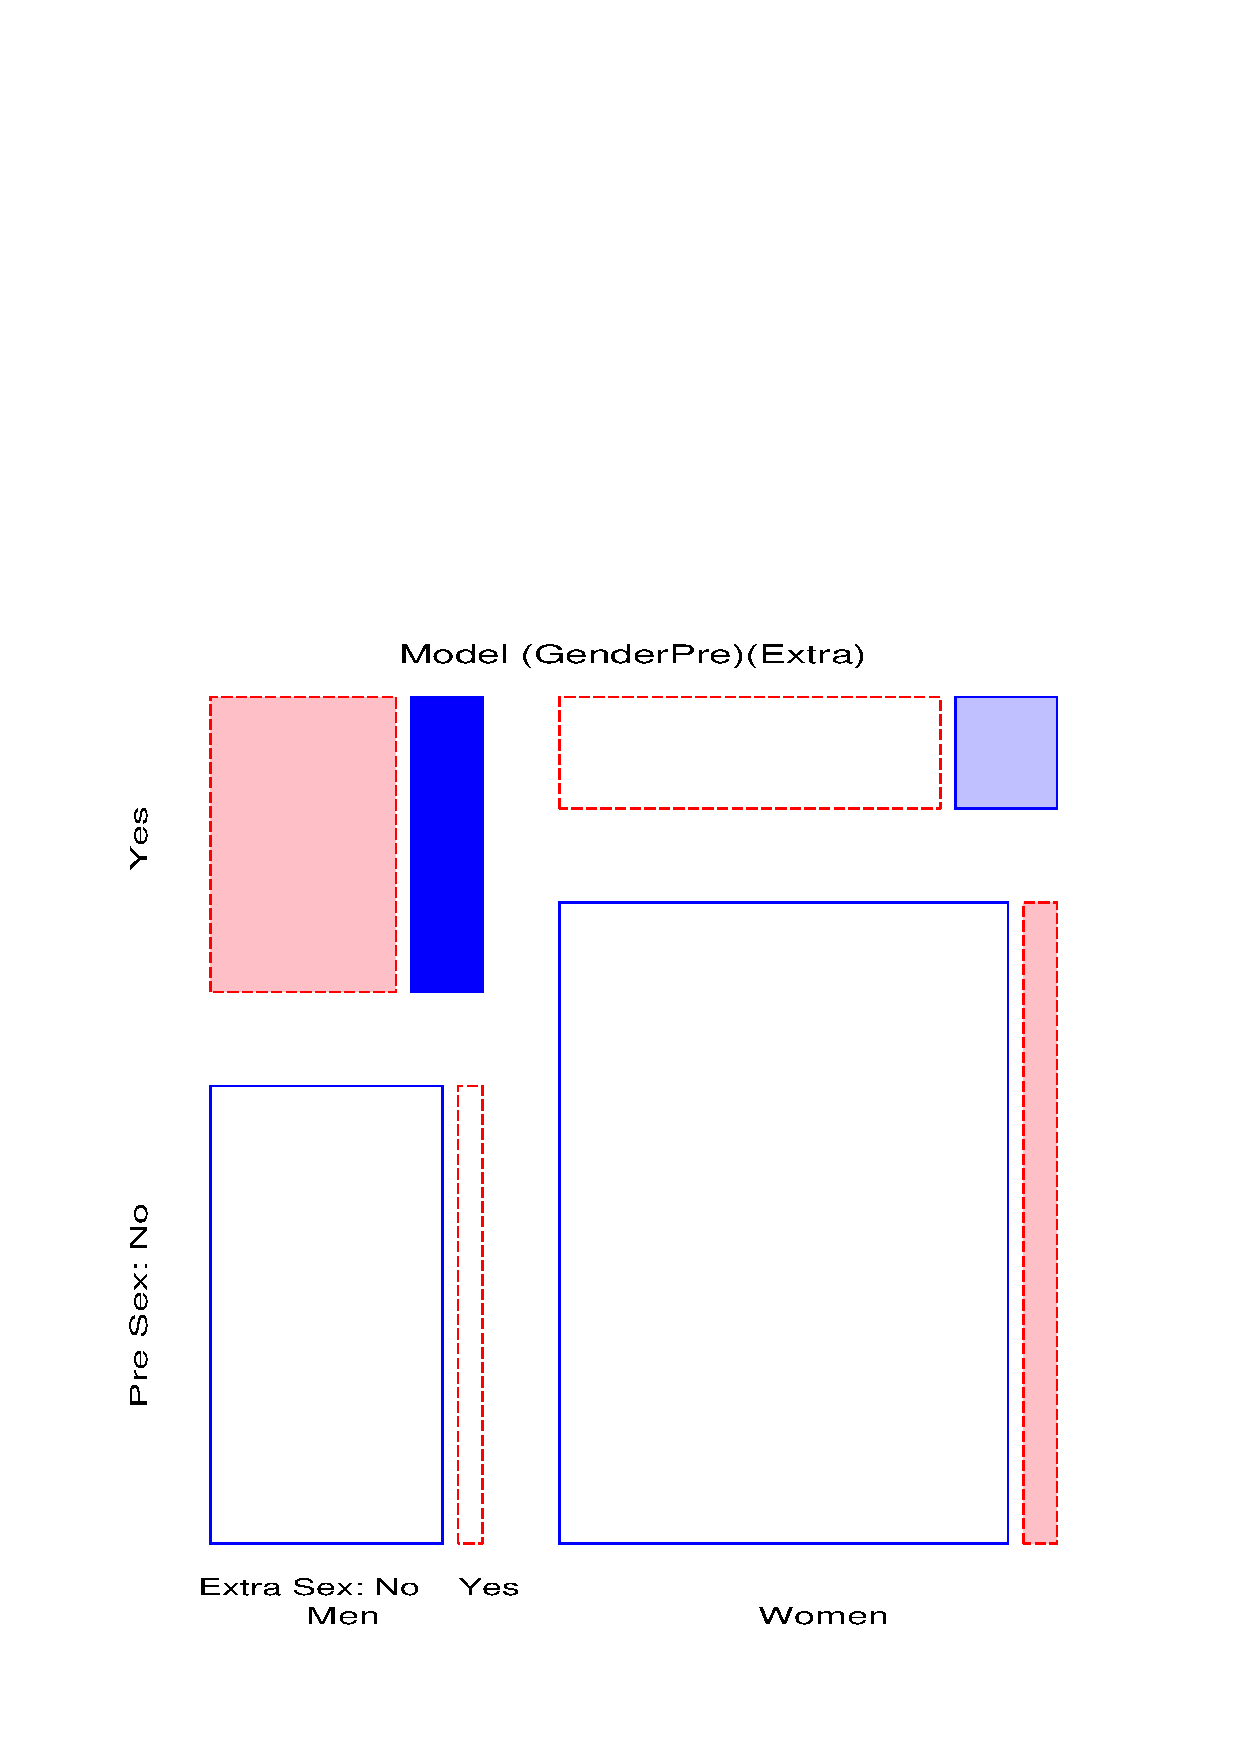
\includegraphics[width=1\linewidth]{ch4/fig/mosaic52}
  \caption[Mosaic display for the model of
joint independence]{Mosaic display for the model of
joint independence, \llmtwo{GP}{E}.}\label{fig:mosaic52}
 \end{minipage}
\end{figure}

For the second stage, the [Gender, Pre][Extra] mosaic is shown in 
\figref{fig:mosaic52}.  \GSQ\ for the model \LLM{GP,E}
is 48.93 on 3 \(df\), indicating that extramarital sex
depends on
gender and premarital sex jointly.  From the pattern
of residuals in \figref{fig:mosaic52} we see that men and
women who have reported premarital sex are far more likely to report
extramarital sex than those who have not.  From the marginal totals
for the [GP] [E] table, the conditional odds ratio of extramarital
sex is 3.61 for men and 3.56 for women.  Thus, extramarital sex
depends on premarital sex, but not on gender.


\figref{fig:mosaic53} shows the mosaic for the final stage, fitting
the model [Gender, Pre, Extra] [Marital].
It shows that
marital status depends
strongly on gender, premarital sex, and extramarital sex jointly.
Among those reporting no
premarital sex (bottom part of \figref{fig:mosaic53}), there
is a similar pattern of cell sizes and deviations for marital status
in relation to gender and extramarital sex:  People who did
not report premarital sexual experience are more likely to
remain married if they report no extramarital sex and more likely
to be divorced if they did.  Among those who do report premarital
sex (top part of \figref{fig:mosaic53}), there is also a similar
pattern of sign of deviations, positive for those who are divorced,
negative for those who are married.

%% two figures side-by-side
\begin{figure}[htb]
 \begin{minipage}[t]{.49\linewidth}
  \centering
  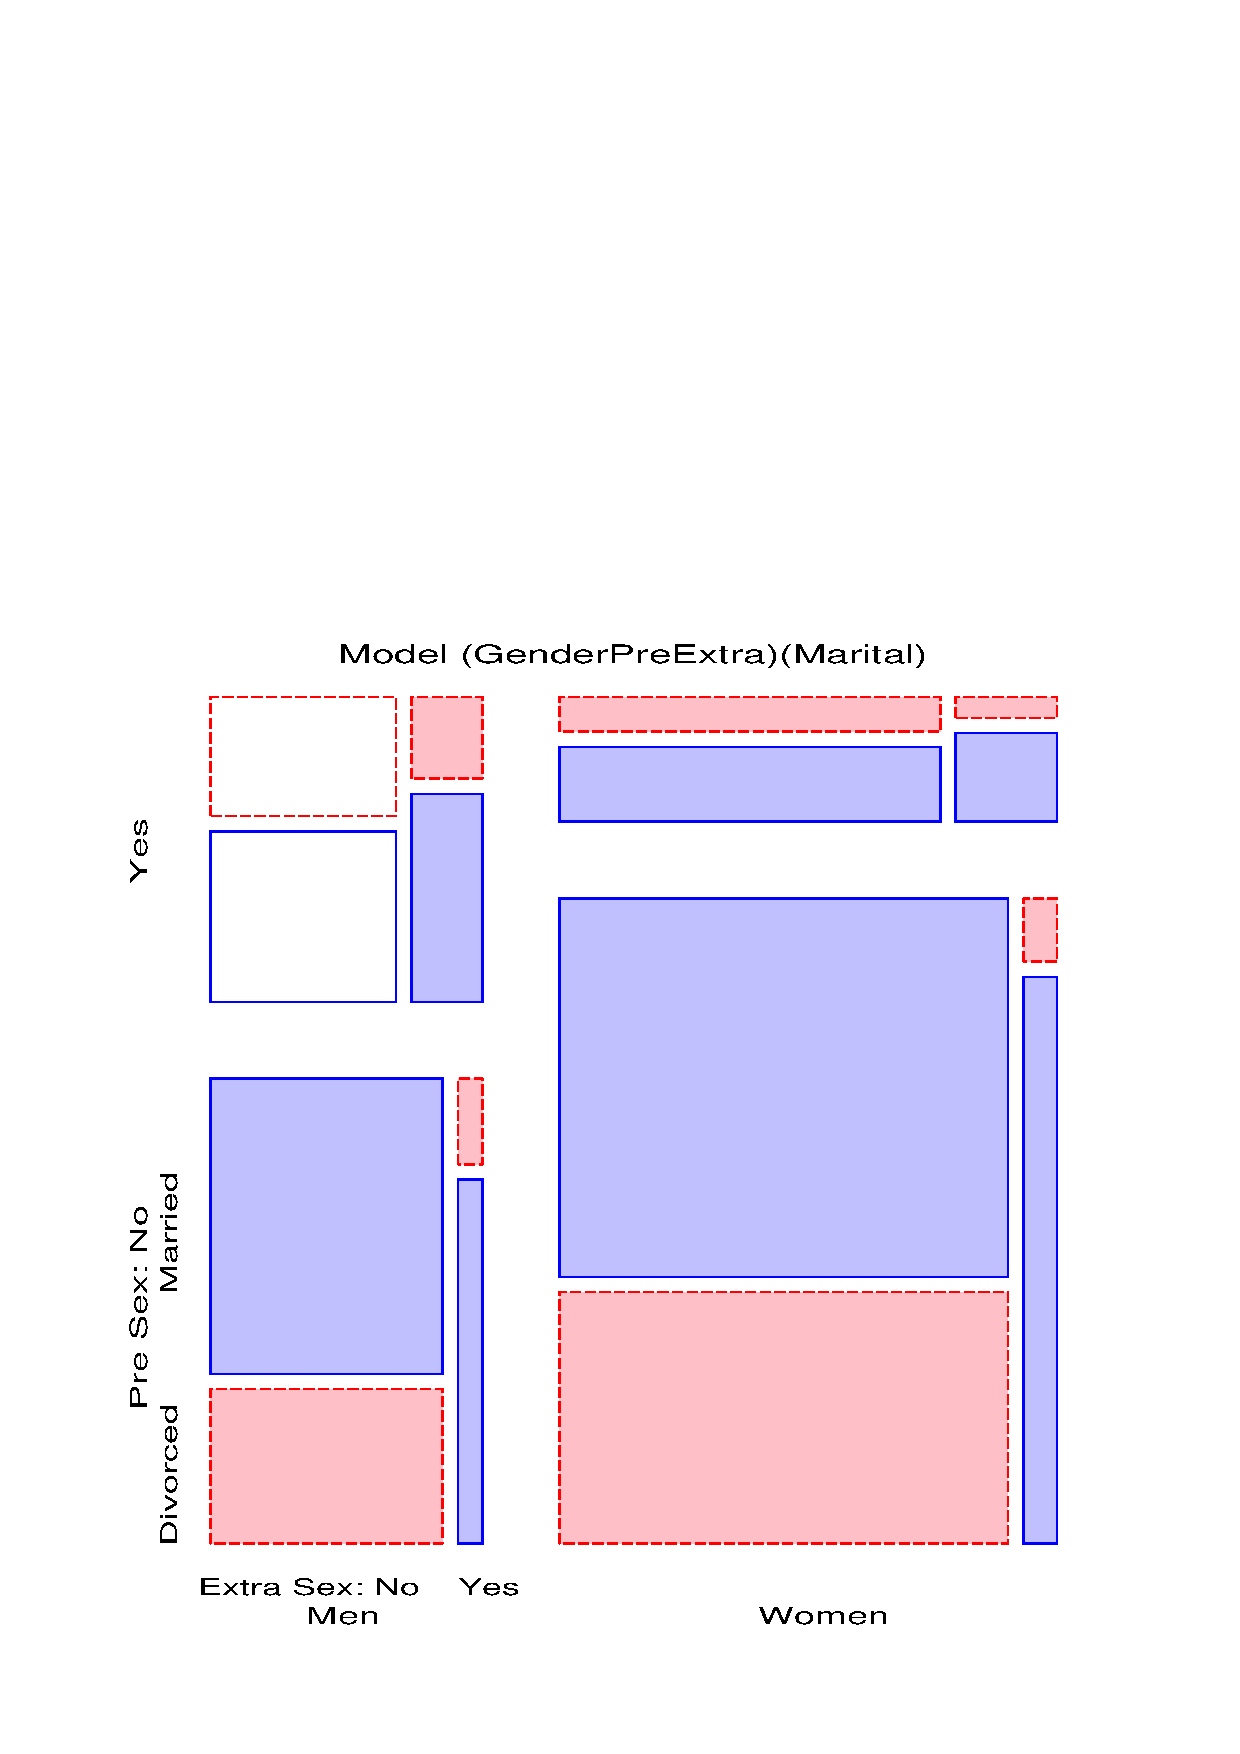
\includegraphics[width=1\linewidth]{ch4/fig/mosaic53}
  \caption[Four-way mosaic for the model \llmterm{GPE} \llmterm{M}]{Four-way mosaic for the model \llmterm{GPE} \llmterm{M}.  The pattern of residuals suggests terms to be included
in an explanatory model.}%
  \label{fig:mosaic53}
 \end{minipage}%
 \hfill
 \begin{minipage}[t]{.49\linewidth}
  \centering
  \includegraphics[width=1\linewidth]{ch4/fig/mosaic54}
  \caption[Four-way mosaic for the model \llmterm{GPE} \llmterm{PEM}]{Four-way mosaic for the model \llmterm{GPE} \llmterm{PEM}.} \label{fig:mosaic54}
 \end{minipage}
\end{figure}

The four \(2 \times  2\) blocks in \figref{fig:mosaic53} show the conditional
relation of extramarital sex to marital status.  Comparing these, we
see that the odds ratios of divorce in relation to reported
extra-martial sex are considerably larger for men and women who also
reported premarital sex.  These observations imply the need to
incorporate associations \llmterm{PM} and \llmterm{EM} of premarital and
extramarital sex with marital status, and probably the three-way association
\llmterm{PEM} into an explanatory model.
Since this stage
considers marital status as a response to gender, premarital sex and
extramarital sex, we would normally fit the $\{GPE\}$ marginal
table exactly, and consider the models \LLM{GEP,PM,EM} or 
\LLM{GPE,PEM} for the complete table.

The model \LLM{GPE,PM,EM} does not fit particularly well
(this mosaic is not shown here),
producing \(G^2  =  18.16\) on 5 \(df\) \(( p  =  .0028 )\).
The model \LLM{GPE,PEM}, however, does  fit quite well, \(G^2  =  5.25\)
with 4 \(df\) \(( p  =  .26 )\).
The term \llmterm{PEM} indicates that premarital sex and extramarital
sex interact in their effects on marital status:
The effect of extramarital sex on divorce is much greater for those
who had no premarital sex than for those who did!
The final mosaic for this model, shown in \figref{fig:mosaic54},
still shows some slight structure in the pattern of signs
of residuals (compare the blocks for men with those for women),
but all residuals are quite small.
\end{Example}